\documentclass[a4paper,runningheads]{llncs}
\usepackage[T1]{fontenc}
\usepackage{graphicx}
\usepackage{booktabs}
\usepackage{amsmath,amssymb}
\usepackage{microtype}
\usepackage{url}
\usepackage{cite}

\InputIfFileExists{generated/macros.tex}{}{}
\providecommand{\PermMaxCarf}{??}\providecommand{\NPerm}{??}\providecommand{\PermPCarf}{??}\providecommand{\PermMeanCarf}{??}
\newcommand{\logit}{\operatorname{logit}}

\pdfinfoomitdate=1
\pdftrailerid{}
\pdfsuppressptexinfo=-1
\begin{document}
\title{Supplementary Material:\\ CARF: Bounded Anchored Fusion for Multimodal Prediction with Unreliable Modalities}
\titlerunning{CARF: Bounded Anchored Fusion (Supplement)}
\author{Anonymous Authors}
\authorrunning{Anonymous Authors}
\institute{Anonymous Institution}
\maketitle

\setcounter{section}{0}
\renewcommand{\thesection}{S\arabic{section}}
\renewcommand{\thetable}{S\arabic{table}}
\renewcommand{\thefigure}{S\arabic{figure}}

\section{Data and preprocessing}

\paragraph{Patient linkage.} Identifiers are matched explicitly across the clinical, expression, imaging, and RPPA sources. The development cohort contains \NDev{} I-SPY2 patients (\NDevPos{} with pCR) with clinical data, expression (GSE194040), and usable pretreatment MRI; RPPA \cite{wolf2022ispy} is available for \NRppa{} of them (\NRppaFeat{} features). The external cohort contains \NExt{} I-SPY1 patients (\NExtPos{} with pCR) with expression (GSE22226) and usable MRI and no RPPA. Expression is restricted to the \NGenes{} shared genes and replaced, for each patient, by within-patient ranks divided by the number of observed genes; missing values are imputed with the training median inside every expert fit.

\paragraph{Treatment-aware anchor.} The anchor is a class-balanced logistic regression ($C=1$) on age, HR status, HER2 status, and four therapy-class indicators derived from the assigned regimen: anti-HER2 antibody (trastuzumab, pertuzumab, or T-DM1), immunotherapy (pembrolizumab), platinum (carboplatin), and HER2 tyrosine-kinase inhibitor (neratinib). In I-SPY1, all patients received anthracycline-based chemotherapy, and the anti-HER2 indicator is set from the recorded regimen (AC+T+trastuzumab); I-SPY1 patients without an expression record (natural-missingness analysis) and GSE25066 patients are assigned no anti-HER2 therapy. The therapy class is fixed before treatment starts and is therefore a legitimate input of a pretreatment prediction under a planned regimen. In a preliminary internal check, subtype-by-therapy interactions did not improve the anchor and were not used.

\paragraph{Experts and auxiliary heads.} RNA: training-median imputation, top 3{,}000 genes by training variance, 250 genes by ANOVA $F$-test, standardization, logistic regression with $C=0.1$. MRI: \NMriFeat{} fixed features (54 signal summaries of the precontrast, early, and late phases and enhancement maps, six shape descriptors, two kinetic fractions, four texture descriptors), median imputation, standardization, $C=1$. RPPA: median imputation, standardization, $C=0.01$; fitted and applied only on patients with RPPA. The auxiliary heads use the same preprocessing (50 ANOVA-selected genes for RNA) and unweighted logistic regressions for HR and HER2 status, fitted on training patients with recorded values. Larger RNA gene sets were screened during development; because I-SPY1 performance informed their rejection, the I-SPY1 results are exploratory rather than an untouched validation.

\paragraph{Verification gate.} For modality $j$ and a patient with recorded HR/HER2 values $c=(c_1,c_2)$, the auxiliary heads give $q_{jt}$, and $\ell_j=\prod_t q_{jt}^{c_t}(1-q_{jt})^{1-c_t}$. The swap likelihood $\bar\ell_j=\frac1N\sum_{i}\prod_t q_{ijt}^{c_t}(1-q_{ijt})^{1-c_t}$ averages over the inner out-of-fold auxiliary predictions $q_{ij}$ of the $N$ training patients with modality $j$, i.e., it is the likelihood of the record if the sample came from a random training patient. The gate $g_j=\pi\ell_j/(\pi\ell_j+(1-\pi)\bar\ell_j)$ with $\pi=0.95$ is a posterior probability in $[0,1]$. In the swap environments of the objective and in the swap stress tests, the auxiliary predictions move with the swapped sample and the gate is recomputed against the receiving patient's record. Pooled over the internal test folds, the gate separates own from swapped samples with AUROC \GateAucRna{} (RNA), \GateAucRppa{} (RPPA), and \GateAucMri{} (MRI); own samples have a gate below 0.5 in \GateLowTrueRna\% (RNA) and \GateLowTrueRppa\% (RPPA) of the cases.

\paragraph{Gated baselines and mix-ups.} Each gated baseline is the corresponding baseline fitted to $\tilde p_j=\sigma(a+g_j(\logit p_j-a))$, where $g_j$ is the verification gate with the training patients' out-of-fold auxiliary predictions as reference, exactly as in CARF; missing experts stay missing. The semi-realistic mix-ups affect RNA and RPPA. \emph{Offset}: the patients with the modality are ordered by GEO accession number, and a contiguous run of 20\% of them (random start) receives the sample of the preceding patient. \emph{Batch}: 20\% of the samples are drawn at random and permuted among themselves within their processing batch (I-SPY2 expression: array platform and normalization method; RPPA: array; I-SPY1: one batch). \emph{Subtype}: all samples are permuted within the three HR/HER2 subtypes. In every mix-up, the auxiliary predictions move with the sample.

\section{Full comparison tables}

Table~\ref{tab:ci} reports paired intervals for the failure average and the worst case of CARF against every comparator. Table~\ref{tab:stress} reports the main failure scenarios, Table~\ref{tab:design} the effect of the anchor and of RPPA, Table~\ref{tab:ablation} the CARF ablations, Table~\ref{tab:internalfull} all internal failure scenarios, Table~\ref{tab:externalfull} all external output-level scenarios, including the extreme and neutral outputs used in training, and Table~\ref{tab:inputfull} all input-level corruption levels. Fig.~\ref{fig:tradeoff} summarizes the trade-off between accuracy on intact inputs and in the worst failure scenario.

\begin{table}[h]
\centering
\caption{CARF minus comparator, failure-average and worst-case AUROC: point estimate and 95\% interval (internal: corrected resampled $t$ over 25 folds; external: 2{,}000 paired patient bootstrap resamples with realizations held fixed). Positive values favor CARF.}
\label{tab:ci}
\setlength{\tabcolsep}{3pt}
\resizebox{\linewidth}{!}{\InputIfFileExists{generated/tab_supp_ci.tex}{}{}}
\end{table}

\begin{table}[h]
\centering
\caption{AUROC under failure of one optional modality (sw.: sample swap; miss.: removed). Internal: mean over 25 folds with 5 realizations each ($n=\NDev$). External: mean of 30 realizations ($n=\NExt$); input-level corruptions are applied to the inputs of the frozen experts. Bold: best fusion model.}
\label{tab:stress}
\setlength{\tabcolsep}{3pt}
\resizebox{\linewidth}{!}{\InputIfFileExists{generated/tab_stress.tex}{}{}}
\end{table}

\begin{table}[h]
\centering
\caption{Effect of the anchor and of the partially available modality. Internal AUROC on intact inputs (mean over 25 folds) for four designs, and internal RNA-swap AUROC and failure average of CARF. Bold: best model per design.}
\label{tab:design}
\setlength{\tabcolsep}{3pt}
\resizebox{\linewidth}{!}{\InputIfFileExists{generated/tab_design.tex}{}{}}
\end{table}

\begin{figure}[h]
\centering
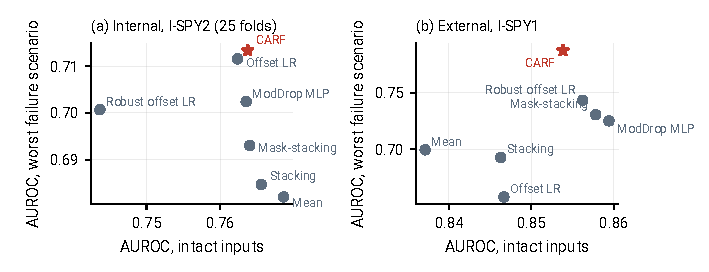
\includegraphics[width=0.9\linewidth]{figures/fig_tradeoff.pdf}
\caption{AUROC on intact inputs versus AUROC in the worst failure scenario, (a) internally and (b) externally.}
\label{fig:tradeoff}
\end{figure}

\begin{table}[h]
\centering
\caption{Ablation of CARF components (treatment-aware anchor, RNA, MRI, and RPPA).}
\label{tab:ablation}
\small
\InputIfFileExists{generated/tab_ablation.tex}{}{}
\end{table}

\begin{table}[h]
\centering
\caption{Internal AUROC (I-SPY2, mean over 25 folds; swap: 5 realizations per fold) for all scenarios.}
\label{tab:internalfull}
\scriptsize
\setlength{\tabcolsep}{3pt}
\resizebox{\linewidth}{!}{\InputIfFileExists{generated/tab_supp_internal.tex}{}{}}
\end{table}

\begin{table}[h]
\centering
\caption{External AUROC (I-SPY1) for all output-level scenarios (swap and noisy: mean of 30 realizations; noisy: Gaussian noise of SD 0.25 on the probability; low/high/neutral: output set to 0.01/0.99/0.5) and the largest displacement from the anchor over all scenarios. R: RNA; M: MRI.}
\label{tab:externalfull}
\setlength{\tabcolsep}{2pt}
\resizebox{\linewidth}{!}{\InputIfFileExists{generated/tab_supp_external.tex}{}{}}
\end{table}

\begin{table}[h]
\centering
\caption{External AUROC under input-level corruption of the frozen experts (mean of 30 realizations): fraction of genes removed, fraction of genes shifted by two log-ratio units, Gaussian noise on the MRI features in training SDs, and fraction of MRI features removed.}
\label{tab:inputfull}
\setlength{\tabcolsep}{3pt}
\resizebox{\linewidth}{!}{\InputIfFileExists{generated/tab_supp_input.tex}{}{}}
\end{table}

\paragraph{Statistical tests.} Internal differences use per-fold paired AUROC differences over the 25 outer folds and the corrected resampled $t$-test with test-to-training ratio $1/4$ \cite{nadeau2003}; the per-fold results of all comparisons are written to \texttt{internal\_paired.csv} by the analysis code.

\section{Additional cohort: GSE25066}

We evaluate the I-SPY2-trained pipeline on GSE25066 without its I-SPY1 samples. For feature compatibility, the RNA expert is refitted on I-SPY2 using only genes shared with GSE25066; no labels from the new cohort are used. MRI and RPPA are absent for all patients. Table~\ref{tab:gse} reports the results.

\begin{table}[h]
\centering
\caption{GSE25066 without its I-SPY1 samples (\GseN{} patients, \GsePos{} with pCR; RNA refitted on I-SPY2 restricted to the shared genes; MRI and RPPA absent). Swap and dropout: mean of 30 realizations.}
\label{tab:gse}
\small
\InputIfFileExists{generated/tab_supp_gse.tex}{}{}
\end{table}

\section{Naturally missing modalities}

Table~\ref{tab:natural} reports the full results for the I-SPY1 patients with naturally missing modalities discussed in the main paper.

\begin{table}[h]
\centering
\caption{I-SPY1 patients with their true availability masks (columns: subset, number of patients/with pCR). ``all'' contains every patient with at least one optional modality; ``partial'' contains patients with exactly one.}
\label{tab:natural}
\setlength{\tabcolsep}{3pt}
\resizebox{\linewidth}{!}{\InputIfFileExists{generated/tab_supp_natural.tex}{}{}}
\end{table}

\section{Calibration}

All experts use class-balanced weights, so all models overestimate the prevalence. Table~\ref{tab:calib} reports calibration on intact inputs; no model is recalibrated.

\begin{table}[h]
\centering
\caption{Calibration on intact inputs (lower is better).}
\label{tab:calib}
\small
\InputIfFileExists{generated/tab_supp_calib.tex}{}{}
\end{table}

\section{Whole-pipeline permutation test}

To test whether the external performance could arise from a pipeline which learns nothing from the development labels, we refit the whole pipeline (experts, auxiliary heads, budget selection, and fusion) on \NPerm{} permutations of the I-SPY2 labels and evaluate on I-SPY1 with the true labels. The external CARF AUROCs have mean \PermMeanCarf{} and maximum \PermMaxCarf{}, compared with the observed \ExtCarfTwo{} ($p=\PermPCarf$).

\bibliographystyle{splncs04}
\bibliography{references}
\end{document}
